\documentclass{report}

\usepackage{color}
\usepackage[usenames]{xcolor}
\usepackage{tikz}

\definecolor{lgray}{gray}{0.9}

\usepackage{listings}

\lstnewenvironment{tsllisting}[1]
{\vspace{3mm}
 \lstset{
    backgroundcolor=\color{lgray},
    basicstyle=\small\ttfamily, 
%    keywordstyle=\bfseries,
    keywordstyle=\underbar,
    identifierstyle=,
    commentstyle=\slshape,
    stringstyle=,
    showstringspaces=false,
    keywords={after,
              always,
              assert,
              assign,
              assume, 
              before,
              bool,
              case,
              choice, 
              cond,
              const,
              controllable, 
              default,
              derive,
              do, 
              else, 
              endtemplate,
              enum,
              export,
              false,
              forever, 
              fork, 
              function, 
              goal,
              if, 
              import,
              init,
              invisible, 
              mem,
              out,
              pause,
              break,
              post, 
              procedure, 
              process,
              return,
              sint,
              stop, 
              struct,
              task, 
              template, 
              true,
              typedef,
              uint,
              uncontrollable, 
              using, 
              void,
              while,
              wait},
    sensitive=false,
    morecomment=[l]{//},
    morecomment=[s]{/*}{*/},
    numberstyle=\tiny,
    stepnumber=1,
    numbersep=1pt,
    emphstyle=\bfseries,
    belowskip=0pt,
    aboveskip=0pt,
    #1
}}{\vspace{3mm}}


\newcommand{\src}[1]{\texttt{#1}}

\newcommand{\tsl}{TSL2 }

\newcommand{\comment}[1]{{\textit{\textbf{#1}}}}


\author{Leonid Ryzhyk}

\title{\tsl Reference Manual}

\begin{document}

\maketitle

\tableofcontents

\chapter{Overview}

\section{Static and dynamic namespaces}

\tsl supports two namespaces: the \emph{static namespace} and the 
\emph{dynamic namespace}.  The static namespace is populated with 
compile-time objects: \emph{types} and \emph{constants}.  The 
dynamic namespace is populated with runtime objects: 
\emph{processes}, \emph{variables}, \emph{methods}, and 
\emph{wires}.  Static objects are uniquely identified by their 
name and syntactic scope.  In contrast, runtime objects can be 
instantiated multiple times within the specification and hence 
must be referred to relative to their runtime scope.  

\section{Templates}

Templates are the principal mechanism for managing both static and 
dynamic namespaces.  A template models an entity, such as a 
device, an OS, or a device driver.  It declares a set of static 
objects (types and constants) and a set of runtime objects.  
Static objects declared inside a template can be referenced from 
any part of the specification via the template name.  Runtime 
objects are instantiated together with the template and can be 
accessed via a reference to a template \emph{instance}.

The following template declares type \src{word} (static object) 
and variable \src{x} (runtime object):
\begin{tsllisting}{}
template A
  // type declaration
  typedef uint<16> word;
  // variable declaration
  export word x;
endtemplate
\end{tsllisting}
The \src{word} type is globally visible via the \src{::}-notation 
as \src{A::word}.  It can be used even if template \src{A} is 
never instantiated.  In contrast, variable \src{x} can only be 
accessed via an instance of \src{A}.  

A template is instantiated inside another template.  The only 
exception is the \src{main} template, which is implicitly 
instantiated in the top-level scope.  Every complete \tsl 
specification must contain a template called \src{main}.  

In the following example, the \src{main} template creates an 
instance of \src{A}, making its variables accessible from 
\src{main} via instance name:
\begin{tsllisting}{}
template main
  instance A a;

  process pmain {
    // assigning variable x of template instance a.
    a.x = 16'd0;
  }
endtemplate
\end{tsllisting}

The template instantiation mechanism gives rise to an 
\emph{instance tree} with the \src{main} template as its root.  
Dynamic objects within the tree are accessed using hierarchical 
names such as \src{a.x}.  This mechanism allows accessing objects 
down the branch of the instance tree, starting at the local 
template.  In practice, it is often necessary to access objects 
instantiated in other parts of the tree.  This is achieved in a 
structured way using \emph{template ports}.  

A template port is an alias to a template of a given type bound at 
the time of instantiation.  For example, template \src{B} below 
declares port \src{aa} of type \src{A}, which makes runtime 
objects in the scope of \src{A} visible from \src{B}.  Both 
templates are then instantiated in the \src{main} template, with 
the instance of \src{A} connected to port \src{aa} of \src{B}.
\begin{tsllisting}{}
// template B with port aa of type A
template B(A aa)
  process proc {
    aa.x = 16'd0;
  };
endtemplate

template main
  // create instances of A and B; connect port aa of
  // B to the instance of A.
  instance A a;
  instance B b(a);
endtemplate
\end{tsllisting}

The following diagram illustrates the resulting instance tree and 
the link between different branches of the tree via port \src{aa}.

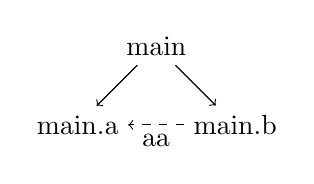
\begin{tikzpicture}
    \node[rectangle] (m) at (0,1) {main};
    \node[rectangle] (a) at (-1,0) {main.a};
    \node[rectangle] (b) at (1,0) {main.b};
    \path[->] (m) edge (a);
    \path[->] (m) edge (b);
    \path[->,dashed] (b) edge node[auto]{aa} (a);
\end{tikzpicture}

Another mechanism for managing name spaces is \emph{template 
inheritance}.  Using inheritance, one can create generic templates 
that capture common properties of a family of entities, leaving 
some of the properties underspecified.  The generic template can 
be specialised by a child template that fills in the missing 
details.  For example, the following template models common 
device-class callbacks that must be implemented by any OS 
specification for the IDE device class.  Note that callbacks are 
defined without bodies, as the exact behaviour is OS-specific.
\begin{tsllisting}{}
template ide_os
  procedure void write_sectors(uint<48> lba, 
    uint<16> sectors, uint<32> buf, bool xfer_error);
  procedure void read_sectors(uint<48> lba, 
    uint<16> sectors, uint<32> buf, bool xfer_error);
  procedure void reset();
  ...
endtemplate
\end{tsllisting}
This template is specialised by the \src{l4\_ide\_os} template,
that describes the IDE driver interface defined by the seL4 OS.
\begin{tsllisting}{}
template l4_ide_os(l4_ide_drv drv)
  // the derive statement is used to establish the 
  // inheritance relation
  derive ide_os;

  // additional specification items can be declared in the 
  // child template
  export iostatus reset_status = ionone;

  // the child template implements methods inherited from 
  // the parent.
  procedure void write_sectors(uint<48> lba, 
    uint<16> sectors, uint<32> buf, bool xfer_error)
  {
    assert (lba == r_lba);
    ...
  }
\end{tsllisting}


\section{Execution model}

All state transitions in \tsl occur in the context of 
\emph{processes}.  Multiple processes can be enabled at the same 
time; however exactly one process participates in each individual 
transition.  Processes are declared inside templates using the 
\src{process} keyword.  Such processes become runnable in the 
initial state of the specification.  Additional processes can be 
spawned at runtime using the \src{fork} construct.  Syntactic 
constraints of the language (namely, the lack of support for 
recursion) guarantee that only a bounded number of processes can 
be spawned at any time.  

In the following example, template \src{A} contains a single 
static process \src{psndrcv}, which spawns two subprocesses 
\src{psend} and \src{preceive}.
\begin{tsllisting}{}
template A

process psndrcv {
  fork {
    psend:    while (true) send();
    preceive: while (true) receive();
  };
  shutdown();
};
...

endtemplate
\end{tsllisting}

%In addition to statically and dynamically created processes, every 
%\tsl specification contains an implicit \emph{idle} 

A process state transition starts in the current program location 
and stops at the next \emph{pause location}.  Pause locations can 
be explicit or implicit.  Explicit pause locations are declared 
using \src{pause}, \src{wait}, and \src{stop} constructs.  
Implicit pause locations are introduced automatically by the 
compiler in the following cases:

\begin{itemize}
    \item Before \src{fork} statements~\ref{}
    \item Before magic blocks~\ref{}
    \item On entries to and exits from controllable and 
        uncontrollable tasks~\ref{}
\end{itemize}

Process behaviour can be factored into \emph{methods}.  A process 
can invoke methods declared inside its own template as well as in 
other template instances, via hierarchical names discussed in the 
previous section.  There are three types of methods in \tsl: 
\emph{functions}, \emph{procedures}, and \emph{tasks}.  Functions 
and procedures must complete instantaneously, i.e., they are not 
allowed to contain explicit or implicit pauses.  In addition, 
functions are not allowed to have side effects, i.e., they cannot 
modify any global variables, perform pointer dereferences, or 
contain assertions (pointer dereferences and assert statements can 
have the side effect of taking the system into an error state).  

Tasks can take time to execute.  A task can have an optional 
\src{controllable} or \src{uncontrollable} qualifier.  
Controllable tasks are the only kind of task that can be invoked 
from synthesised code; although they can also be called from 
manually written code.  They are used to model the device register 
interface and OS callbacks.  Controllable tasks are subject to 
additional implementation constraint.

Uncontrollable tasks represent driver methods invoked by the OS or 
the device.  Uncontrollable tasks are the only kind of task that 
can contain automatically generated code, i.e., a magic block can 
only be placed inside an uncontrollable task.  

Controllable and uncontrollable task invocations introduce 
implicit pause locations on entry and return from the task.  In 
the following example execution of process \src{p1} will consist 
of three transitions.
\begin{tsllisting}{}
template A
  uint<16> x;

  process p1 {
    x=1;
    t1(x);
  };

  task uncontrollable void t1(uint<16> arg) {};
endtemplate
\end{tsllisting}
The first transition assigns global variable \src{x} and sets the 
argument of task \src{t1} to be equal to \src{x}.   An implicit 
pause location is inserted at this point.  The second transition 
executes the body of task \src{t1}, which completes 
instantaneously, as it does not contain any pause locations.  
Another implicit pause is inserted at the task return location.  
The remainder of the process is executed in the third transition.  
Note that other processes can run and potentially modify variable 
values in between transitions 1 and 2 and transitions 2 and 3.

Tasks without \src{controllable} and \src{uncontrollable} 
qualifiers behave as if the body of the task was inlined at the 
call location.  No additional pauses are inserted before or after 
the task.

\section{Variables and wires}

\emph{Variables} are used to store state that persists for the 
lifetime of the variable.  Variables in \tsl can be declared in 
the template, process, or method scope.  Template-scope variables, 
also called \emph{global variables}, are instantiated together 
with the template and are visible from anywhere inside the 
template.  In addition, variables declared with the \src{export} 
qualifier can be accessed from other templates via their 
hierarchical names.  Process and method variables are only visible 
within the syntactic scope of the process or method where they are 
declared.

In contrast to variables, \emph{wires} are simply aliases to 
expressions defined over global variables and are not allocated 
their own storage.  Wires keep their values throughout a 
transition and are updated at the end of the transition.  Initial 
value of a wire is computed based on initial values of global 
variables.

\begin{tsllisting}{}
template A
  uint<16> x = 0;
  wire uint<16> w = x + 1;
endtemplate
\end{tsllisting}


\section{Correctness specifications}\label{s:o:correctness}

\tsl provides several mechanisms for specifying correctness 
conditions over system behaviour:
\begin{itemize}
    \item \emph{Goals.} A goal is a boolean expression over global 
        variables that must hold infinitely often in any infinite 
        run of the system.  A template can declare any number of 
        goals.  In addition, \tsl defines two implicit goals.  The 
        first one requires the system to be outside of a magic 
        block infinitely often; in other words, the system cannot 
        stay inside a magic block forever.  The second implicit 
        goal requires that the system never enters an \emph{error 
        state} (see below).
    \item \emph{Assertions.}  An \src{assert} statement can be 
        placed anywhere inside processes, tasks, and procedures.  
        It defines a condition whose violation immediately 
        transitions the system to an error state.
    \item \emph{Postconditions}.  Magic block postconditions are 
        discussed in Section~\ref{s:o:magic} above.
\end{itemize}



\section{Magic blocks}\label{s:o:magic}

A \emph{magic block} is a place holder for automatically generated 
code.  \tsl supports two types of magic blocks.  Magic blocks with 
\emph{postconditions} specify a condition that must hold upon 
returning from the magic block.  

%Note that for synthesis to succeed the resulting system must 
%satisfy all correctness conditions described in the following 
%section, and not just magic block postconditions.

\begin{tsllisting}{}
template main
  task uncontrollable bool probe() {
    // Magic block with postcondition
    {...} post((os.reset_status == iosuccess) ||
               (os.reset_status == ioerror));
    if (os.reset_status == iosuccess) {
      return true;
    } else {
      return false;
    };
};
endtemplate
\end{tsllisting}

The second type of magic blocks are magic blocks with 
\emph{goals}.  These are needed because not all correctness 
conditions can be captured using postconditions and assertions.  
For correctness conditions specified using goals (see 
Section~\ref{s:o:correctness}), the synthesis algorithm computes a 
strategy for each goal; however the scheduling of strategies is 
left to the user, i.e., the user decides when to execute each 
strategy by assigning goals to magic blocks. \comment{TODO: I 
still have not figured out the exact meaning of this construct.}

%\section{Constraints on the environment}

\chapter{Syntax reference}


\section{Import statements}

Import statements are used to combine multiple \tsl files into a 
single specification.  They are only allowed in the top-level 
syntactic scope, i.e., they are illegal inside template of type 
declarations.  An import statement consists of the \src{import} 
keyword followed by file path in angle brackets:
\begin{tsllisting}{}
import<ide_dev.tsl>
import<os/ide_tsl2/l4_ide.tsl>
import<../../os/ide_tsl2/ide_class.tsl>
\end{tsllisting}
The \tsl compiler appends this path to each import directory, 
specified via the \src{-I} command line switch, in order, until a  
file with this name is found.


\section{Templates}

Templates must be declared within the top-level scope, i.e., 
nested template declarations are not allowed.  Template 
declaration has the following syntax:
\begin{tsllisting}{}
template <template-name>[(<port-declarations>)]
  <template-item>*
endtemplate
\end{tsllisting}



\end{document}
